\subsection{Active Session}
Admins or student assistants have a selector on the main admin dashboard for selecting a session. If there are no sessions, the user will be prompted to create one. After the user has selected a session the start button will be enabled. Pressing this button sends a request to the server requesting this session to be initialized. The server will then proceed to request information from the database of the session. Information of the session is stored as an object in a map. After the server has made the session ready, it will send a response back to the client and switch the view to a waiting room. The waiting room shows a code that students can use to connect and also display the current number of student connected. 
\\[11pt]
On the main client dashboard, there is an option to join an active session. Once a client has joined a session, the user also joins a room in Socket.IO. This is a feature that allows the server to send a message to all clients connected to that room and is used when the session is going from the waiting room to a question, or to the next question. When the admin sends a start signal, the server retrieves information for the next question and send a message to all clients connected to that room.

\begin{figure}[H]
	\centering
	\begin{subfigure}{\linewidth}
		\centering
		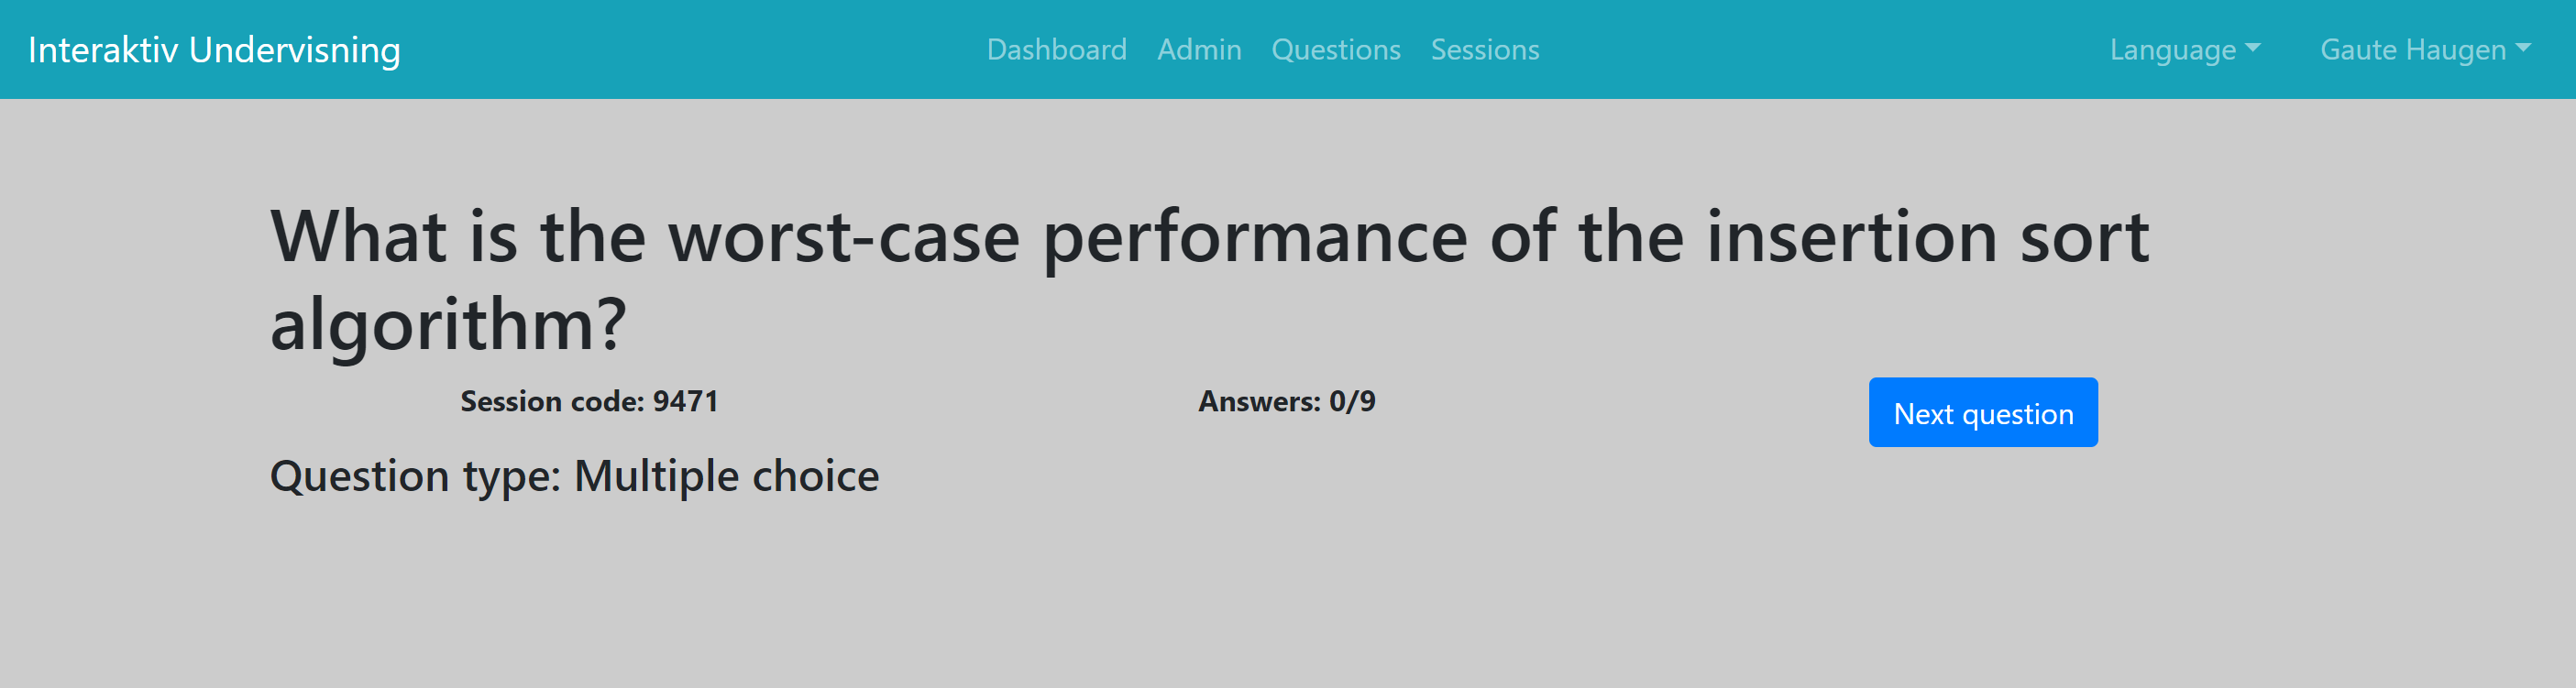
\includegraphics[width=0.80\linewidth]{/userManual/admin/activeSessionQuestion}
		\caption{This is the client side.}
		\label{fig:activeSessionAdmin}
	\end{subfigure}
	\begin{subfigure}{\linewidth}
		\centering
		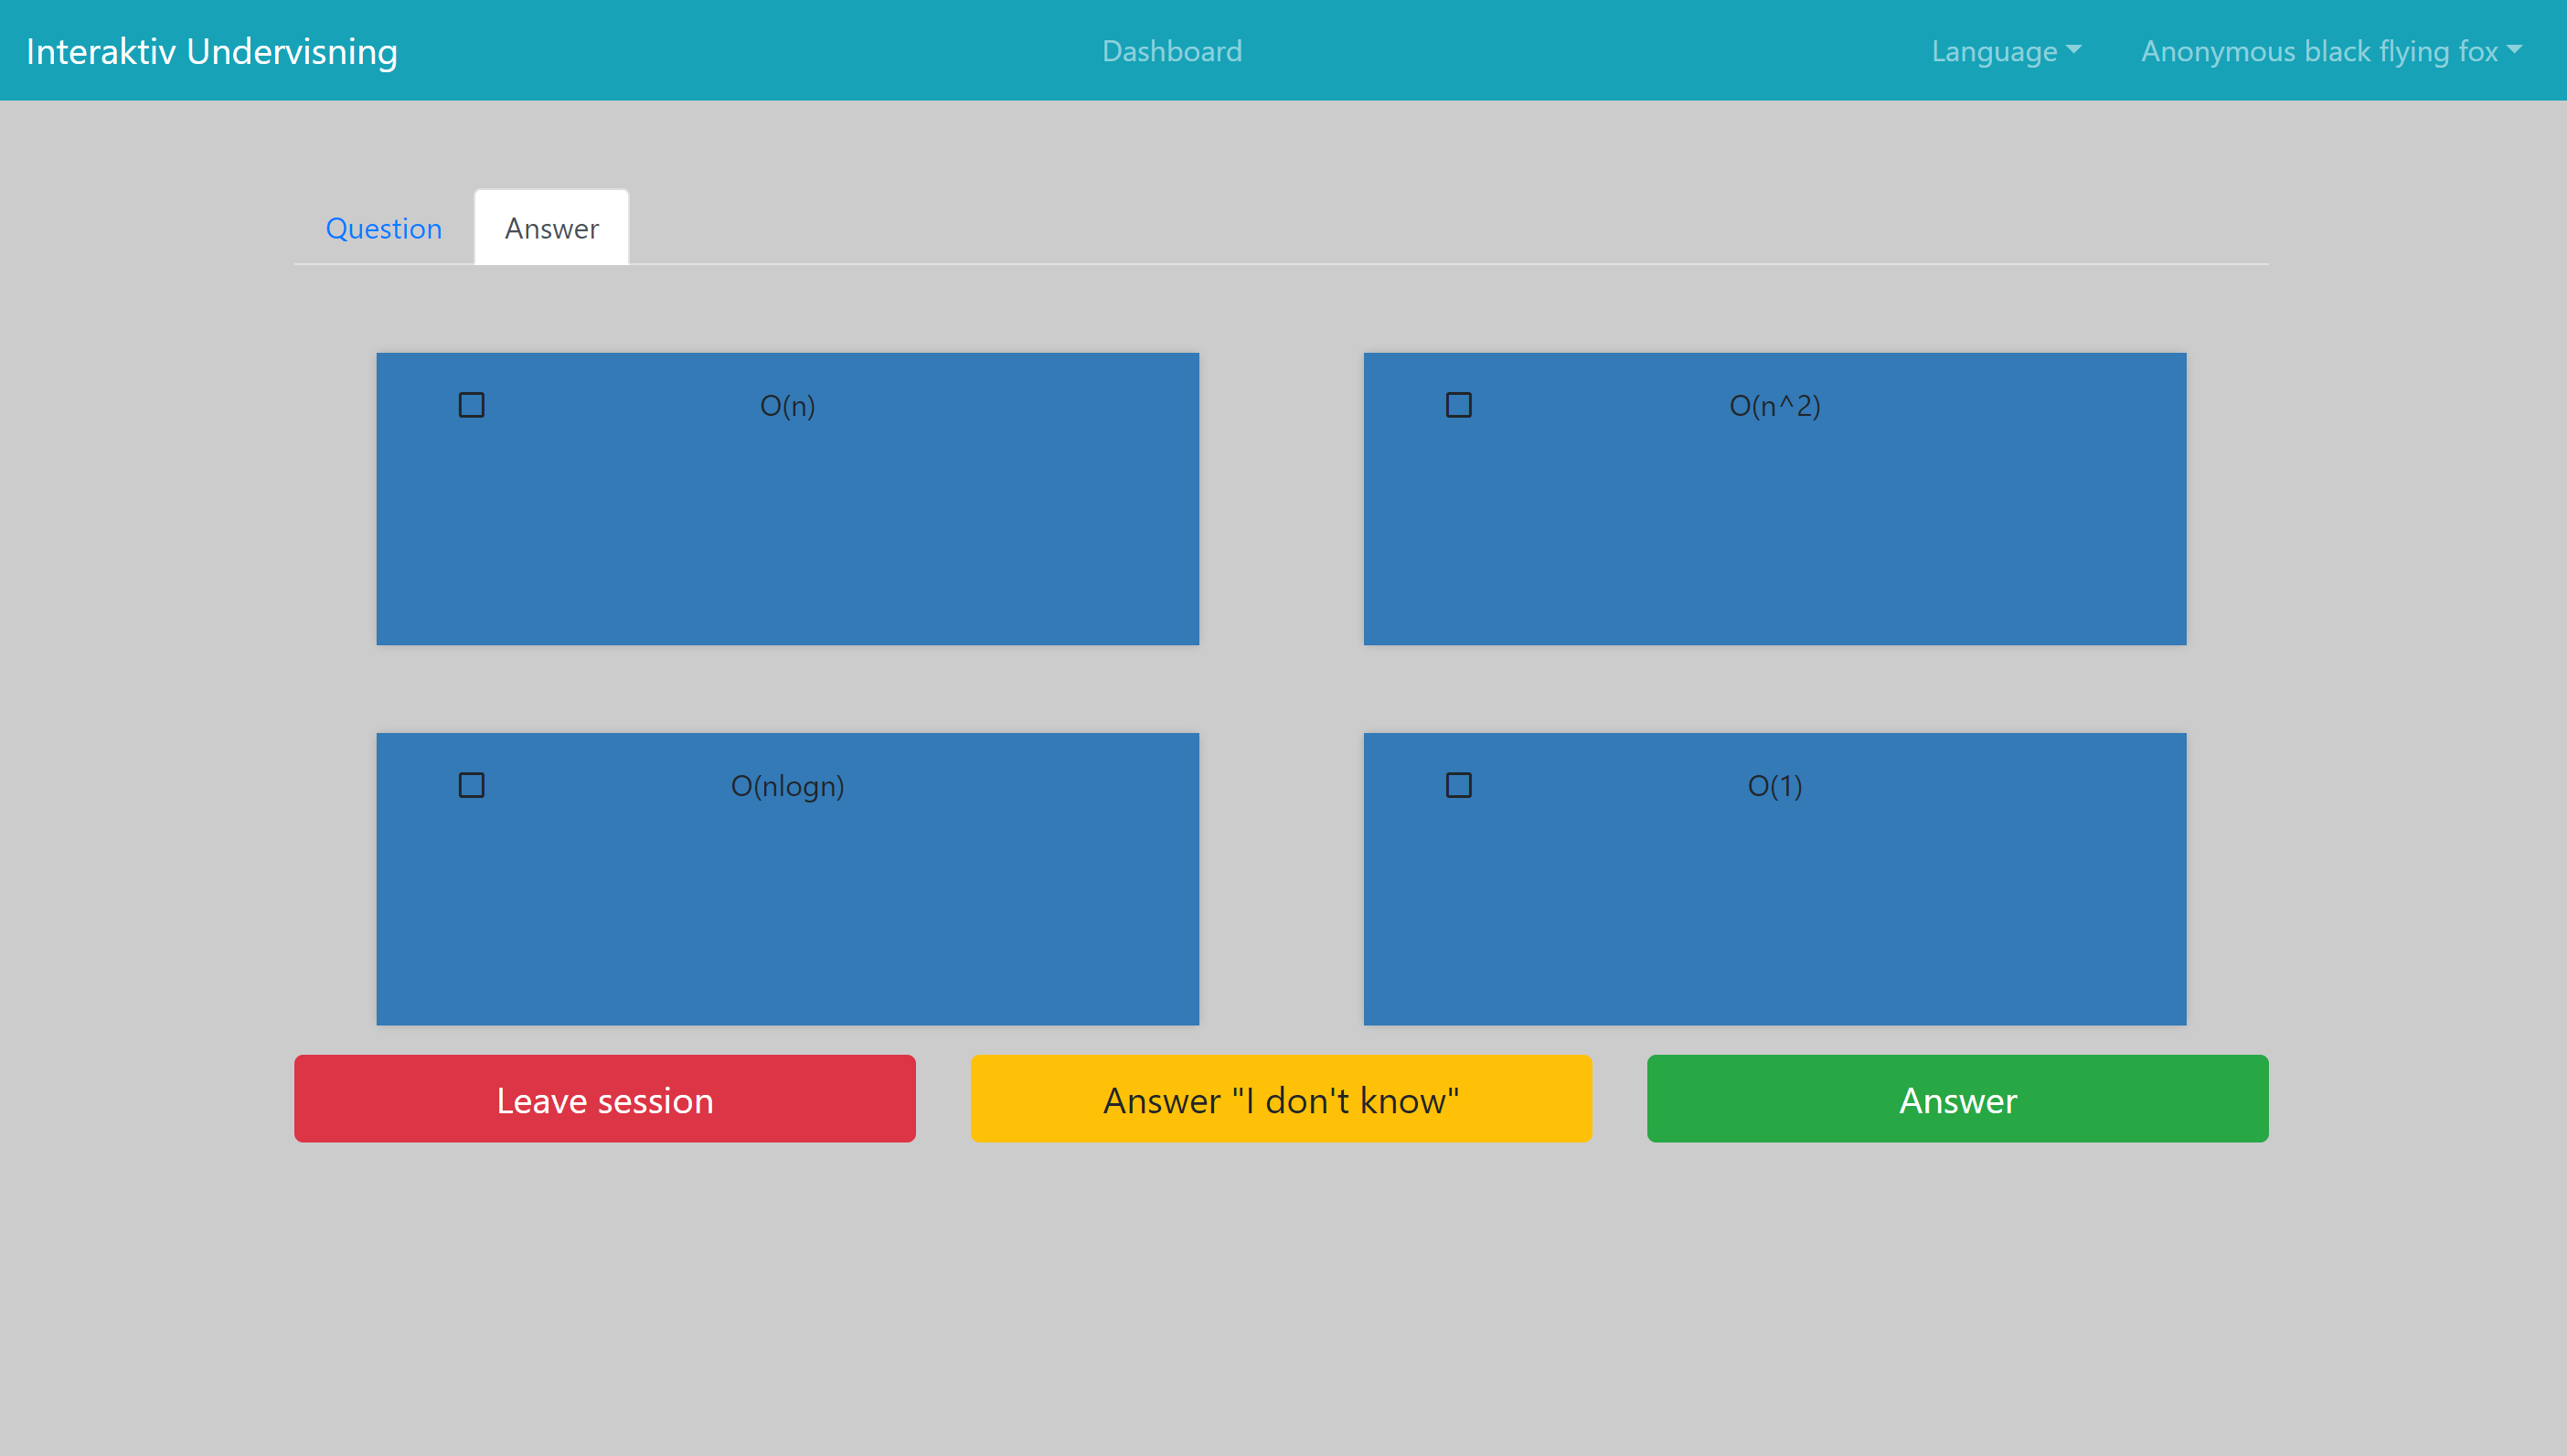
\includegraphics[width=0.80\linewidth]{/userManual/admin/activeSessionClientAnswer}
		\caption{This is the host side.}
		\label{fig:activeSessionClient}
	\end{subfigure}
	\label{fig:activeSession}
	\caption{These figures display a question during an active session.}
\end{figure}

\noindent
When a student receives a message with a question, the active session component switches to a component made to display a question. There is also a similar component for the admin, but they differ as they need other features. When the question component for a student is first shown, the answer tab is displayed, but the student can switch to see the question. This was done in an effort to give students the possibility to view each question if the display in front of the class is hard to see. When a student is on the answer tab, there is a component allowing the student to give their answer in a way that is specific for that question type.
\\[11pt]
When a user sends in their answer, it is sent to the server, where it goes through a solution checker. When using the solution checker, the main script needs the answer, solution, and question type. When getting to the main script, it looks at the question type and then sends the answer and solution to the correct checker. There is a solution checker for each question type, and it will go through the answer and compare it with a solution. The comparison will depend on the question type, but in general, it will loop through the solution and compare the current loop step with what is in the answer. The current solution checker structure can be seen in figure \ref{fig:serverStructure}, where the main script is called "Solution generator" and then all the sub scripts are for each question type. This not only makes it easy to expand with new question types but also makes the debug for solution checking easier.
\\[11pt]
When the server is finished with the solution checker, it sends a message back to the student moving them to a waiting screen with the result. The result will be shown as text and will be as discreet as possible. While the student is transferred to the waiting area the server sends a message to the host of the session informing how many users have answered the question. Once every student has answered the question, the server stores the answers in the database.

\begin{figure}
	\centering
	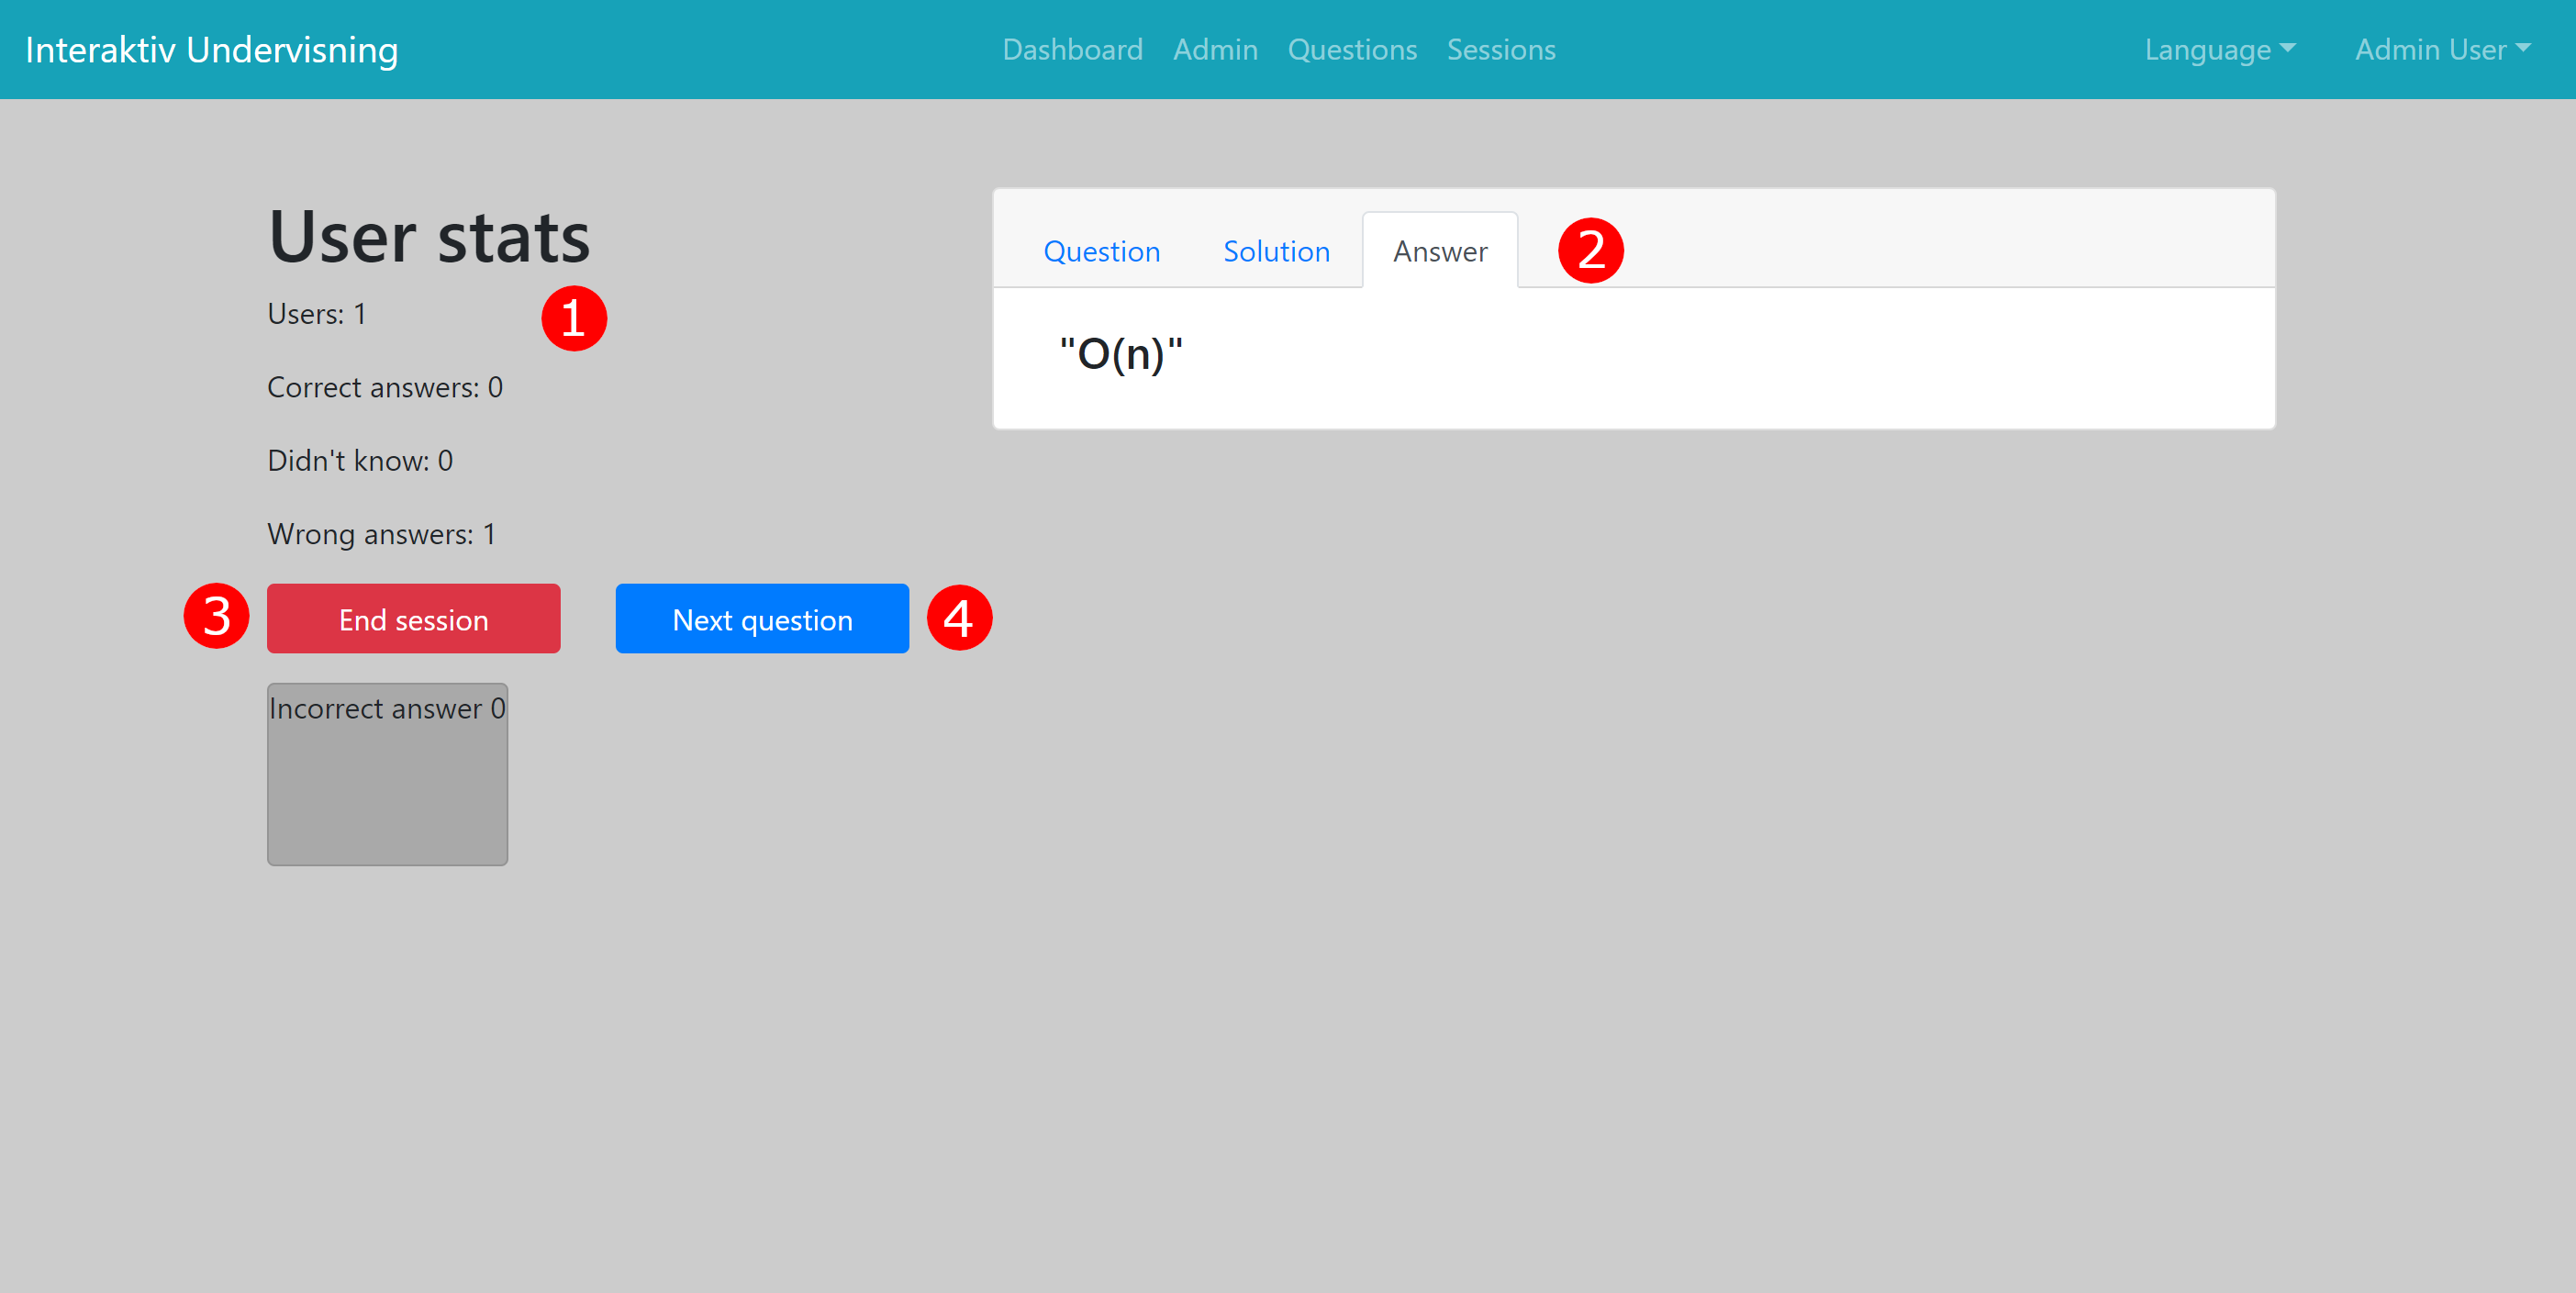
\includegraphics[width=0.80\linewidth]{/userManual/admin/activeSessionResultScreen}
	\caption{The figure displays the result screen of a question.}
	\label{fig:resultScreen}
\end{figure}

\noindent
There are three ways for the session to move on from a question. If all the users connected to the session have answered the question it will move on, if the timer runs out or if the host presses the next button. All students are still in the waiting area, while the server sends statistics and all the wrong answers with the solution to the host. The host is shown basic statistics and a list of all wrong answers, where the host is able to compare the wrong answer with the solution. When the host is ready for the next question there is a button to press to move on. This sends a request to the server requesting the next question, and if there is a new question it is sent out to all students connected to the room and the host. When there is no question left, an end screen is shown for both the students and the host informing them that the session is now over and giving them a button to return to the dashboard.
\\[11pt]
If a user leaves or joins an active session, a message is sent to the server requesting the appropriate event. Leaving a session triggers the following events:
\begin{enumerate}
    \item The server will first check if the user has answered the question or not. 
    \item The server uses different counters to keep track of users during a session. This is done to make sure the counter on the host screen shows the correct amount of answers and users. It is also used to go to the result screen when all users have answered. When a user leaves the correct counters will update
\end{enumerate}
Joining a session triggers the following events:
\begin{enumerate}
    \item The server will first check if the user has answered the question or not, and send them to either the waiting room or to the question.
    \item The counters are updated.
\end{enumerate}
If the host loses connection, refreshes the page or leaves the page, an interval starts, giving the host five minutes to reconnect. No student is kicked out and can answer the current question. If the host does not reconnect, the session is removed as an active session, and all students are moved to the end screen. During these five minutes, a host can not start a new session and can rejoin the session or clear it. Clearing the session ends the session and sends all connected users to the end screen.